\section{Agile planning}

The project was preceded by the search for a subject. This search has been
related to the initial plan of adding multiplayer functionality to an existing
tour app, GeoQuest. As the search lengthened, the focus diverged from the
tour app, towards GPS-enabled multiplayer games. The first ideas were for
including including small games and side activities into the tour app.
During three months, several GPS-enabled mobile games have been tried out.
Ideas from before 2007(the first iPhone) have also been scouted, along with
existing games on both Google Play and Apple's App Store. Besides that, sports
such as orienteering have been used as inspiration.\newline

The games that were found either required too much or too little involvement
from the players, required no actual movement or demanded the player to go to various
locations alone just to progress in the game. The point of this project has
become making a game that would entertain a number of people that would play
together, without the need of specific skills, know-how or prolonged
involvement. It would be played within at most 30 minutes.\newline

From all the previous ideas, the 'War Game', 'Mine Game' and 'Territory
Takeover' games were proposed. From all three, the 'War Game' was chosen for
development, while the other two have been kept for future work. On the 14th of
January, at the end of the three month exploration phase, the work has
started.\newline

In the proposal for the project, the 6 month time has been separated in four
parts :

\begin{enumerate}
  \item \textbf{First phase of development - 2 months}: During the first
  iteration of development, the most basic features of the game were to be
  implemented: basic server functionality that would allow the game to work,
  basic client functionality and the 'War Game' with the most basic features.
   
  \item \textbf{First phase of testing - 1 month}: During this phase, the game
  and its functionality would be live-tested for feasibility and quality. New
  ideas would be sought and documented. Most importantly, player feedback would
  be gathered. 
  
  \item \textbf{Second phase of development - 2 months}: During the second
  iteration of development, the 'War Game' would be completed and, using its
  framework, the 'Territory Takeover' game would be implemented. Bugs would be
  removed and tweaks would be made to the framework and the game concepts to
  match the player feedback.
  
  \item \textbf{Second phase of testing - 1 month}: During the second evaluation
  phase, both games would be tested for playability, player feedback would be
  gathered and the written paper would be completed.
\end{enumerate}

This schedule has proven unfeasible - not because of the length of the
development phases, but because of the very short length of the testing phases.
It has also been concluded that implementing two game concepts would only
greatly reduce the depth of research and would most likely provide incomplete
user experiences. The 'Territory Takeover' game has been left as future
work. Another big part of the development of this app has been played by the
continuous search for the appropriate technologies and practices for the project
- including organizing:

\begin{enumerate}
  \item The exploration phase - Creating a UI test (Android), a server test
  (in NodeJS, then Python, then Java), a client test(Android). There have also
  been some short UI tests and discussions along the way. This phase took around
  two-three weeks.
  
  \item The initial development phase - Creating a functional app with the Maps
  API V1 and writing a full-blown server. This was the longest phase - taking
  around one month and a half. No compatibility libraries were used, and
  therefore the app required Android versions of 3.0 or higher.
  
  \item The first testing phase - It lasted for half a day. Preparations for it
  took another few hours (upgrading the OS on two phones from Android 2.3 to
  4.0). A few friends of the author volunteered their Android devices.
  The application has been installed on all their phones and tried out for one
  hour (in multiple attempts, with some crashes). After playing the game, a
  focus group - style discussion was set up, the subjects being the usability,
  mechanics and feeling in and out of the game. Notes were taken, while
  everybody was discussing various aspects of the app. Also the menus and a
  possible logo were discussed. Even though the time has been short, enough
  input was gathered to change the appearance and workings of the application
  almost completely. Also this is when the decision has been taken to make the
  app compatible with Android 2.3 for the least (almost 50\% of Android users
  had this version on their phones at the time).
  
  \item The second development phase - Another three weeks were required to
  completely construct a new UI according to the requirements from the testing
  phase and the switch from Google Maps API V1 to V2. Crash logging and data
  usage logging have been added to the app.
  
  \item The second testing phase lasted one day. This time, the number of the
  people who participated has doubled - ten people. Most of them also had 3G sim
  cards. The game was finally field tested. Another focus group - style
  discussion has been set up and the opinions and suggestions were noted down.
  
  \item The documentation phase is ongoing. This is the paper documenting the
  development of the app.
  
\end{enumerate}

\subsection{Kanban}

For managing the development steps of the app, a simplified Kanban board was
mainly used. As is specific to Kanban, stories have been gradually proposed and
fragmented them tasks, where necessary. As the work for this project has been
solo, all team aspects of this organizational system have been removed. The
fields that have been kept are an 'Input Queue' of three slots, two
'Development' slots, two 'Integration' slots and three 'Live slots'.\newline

This board has been custom made for this project, unlike the typical Kanban
board - a whiteboard with slots defined by lines drawn with a marker, on which
the stories and tasks were held with magnets. The custom approach to make the
board, even though more time consuming, has proven more efficient for the
long term of the development of this application. When a whiteboard is used,
stories and tasks and magnets are lost - losing stories is something this
project cannot afford. The markers get misplaced and paper is often not found.
For the development of the app, the Kanban board was made out of an actual
wooden board, on which transparent plastic envelopes of two different sizes were
placed as slots for the stories and tasks. Also, under the board, three more
slots have been added : one for the papers for the stories and tasks, one for
the utensils(markers and pens of various colors and scissors) and the last one
for the finished stories and tasks that did were pushed outside the board. This
gave better control over the location of everything needed and multiple stories
could be placed in the same slot. For example, the two 'Input Queue' slots have
proved to be not enough for the influx of ideas and proposals for modification.
Also, the 'Live' slots were not used for single stories, but for groups, as will
be described below. The Kanban board can be seen in Figure \ref{fig:kanbanBoard}.Its
extension is presented in Figure \ref{fig:kanbanBoardExtension}.\newline

\begin{figure}
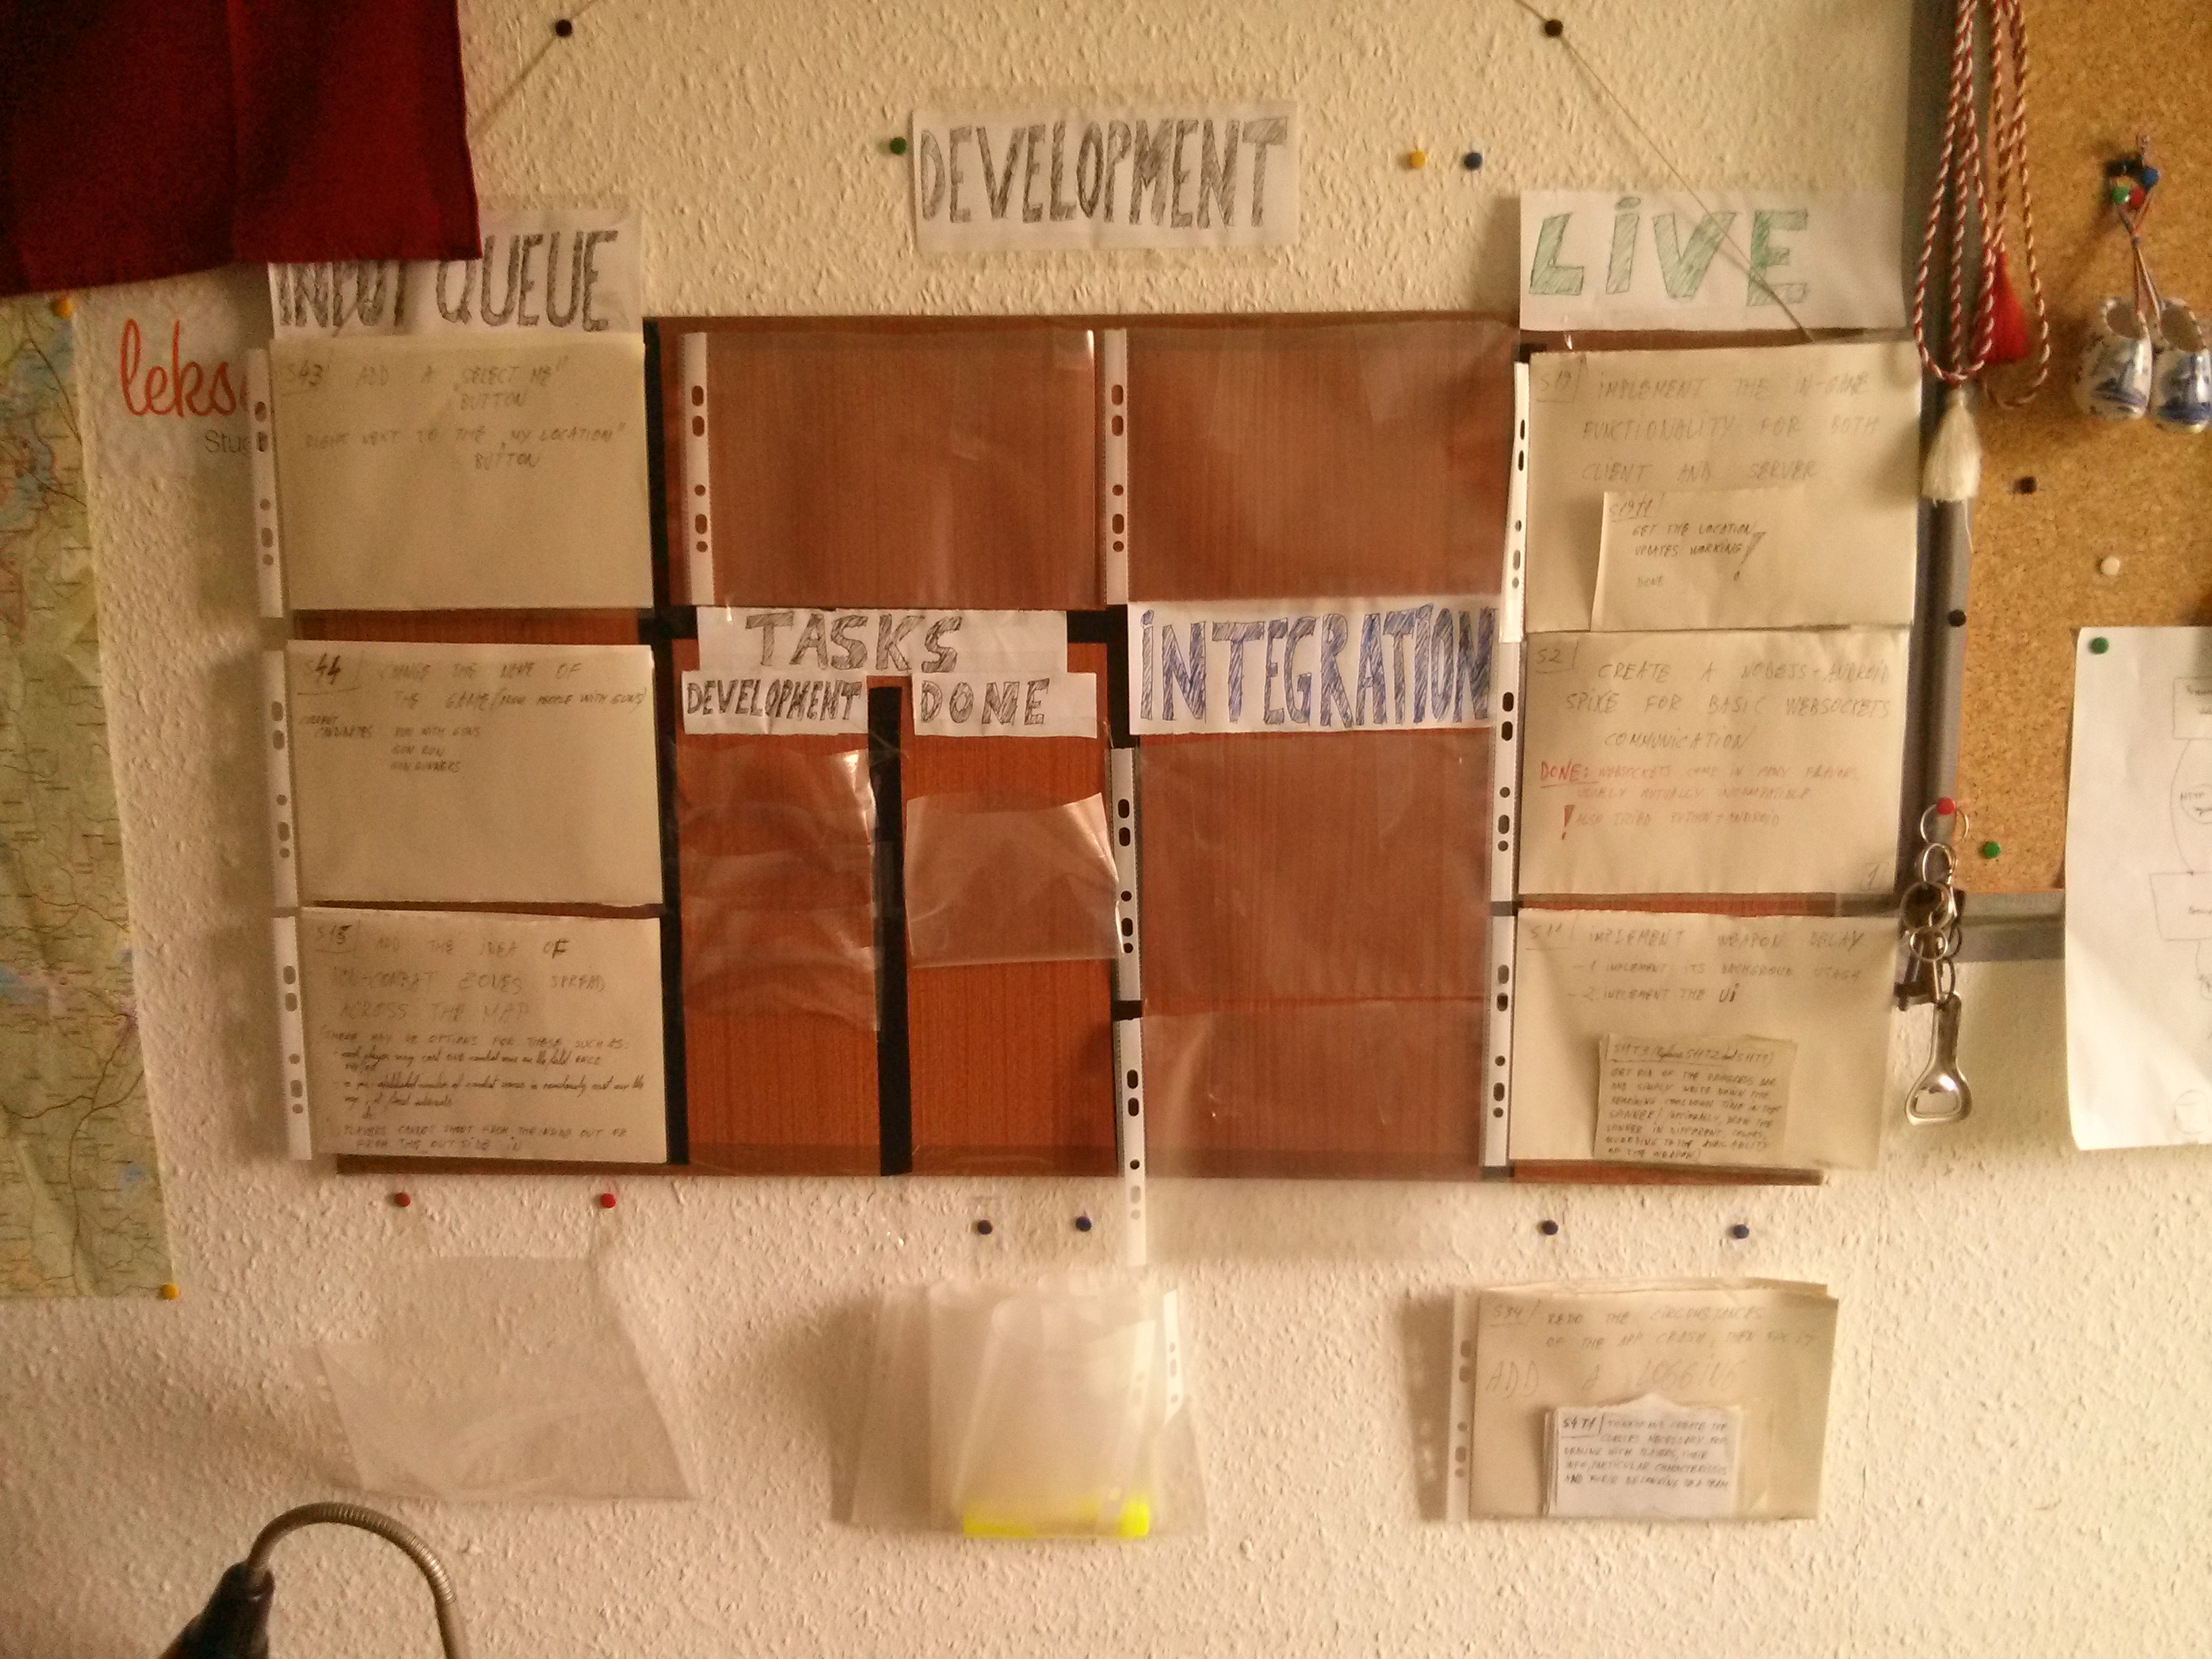
\includegraphics[height=3.5in,width=6.23in]{./images/kanban/kanban_board.jpg}  
\caption{\small \sl Kanban board \label{fig:kanbanBoard}}
\end{figure}

\begin{figure}
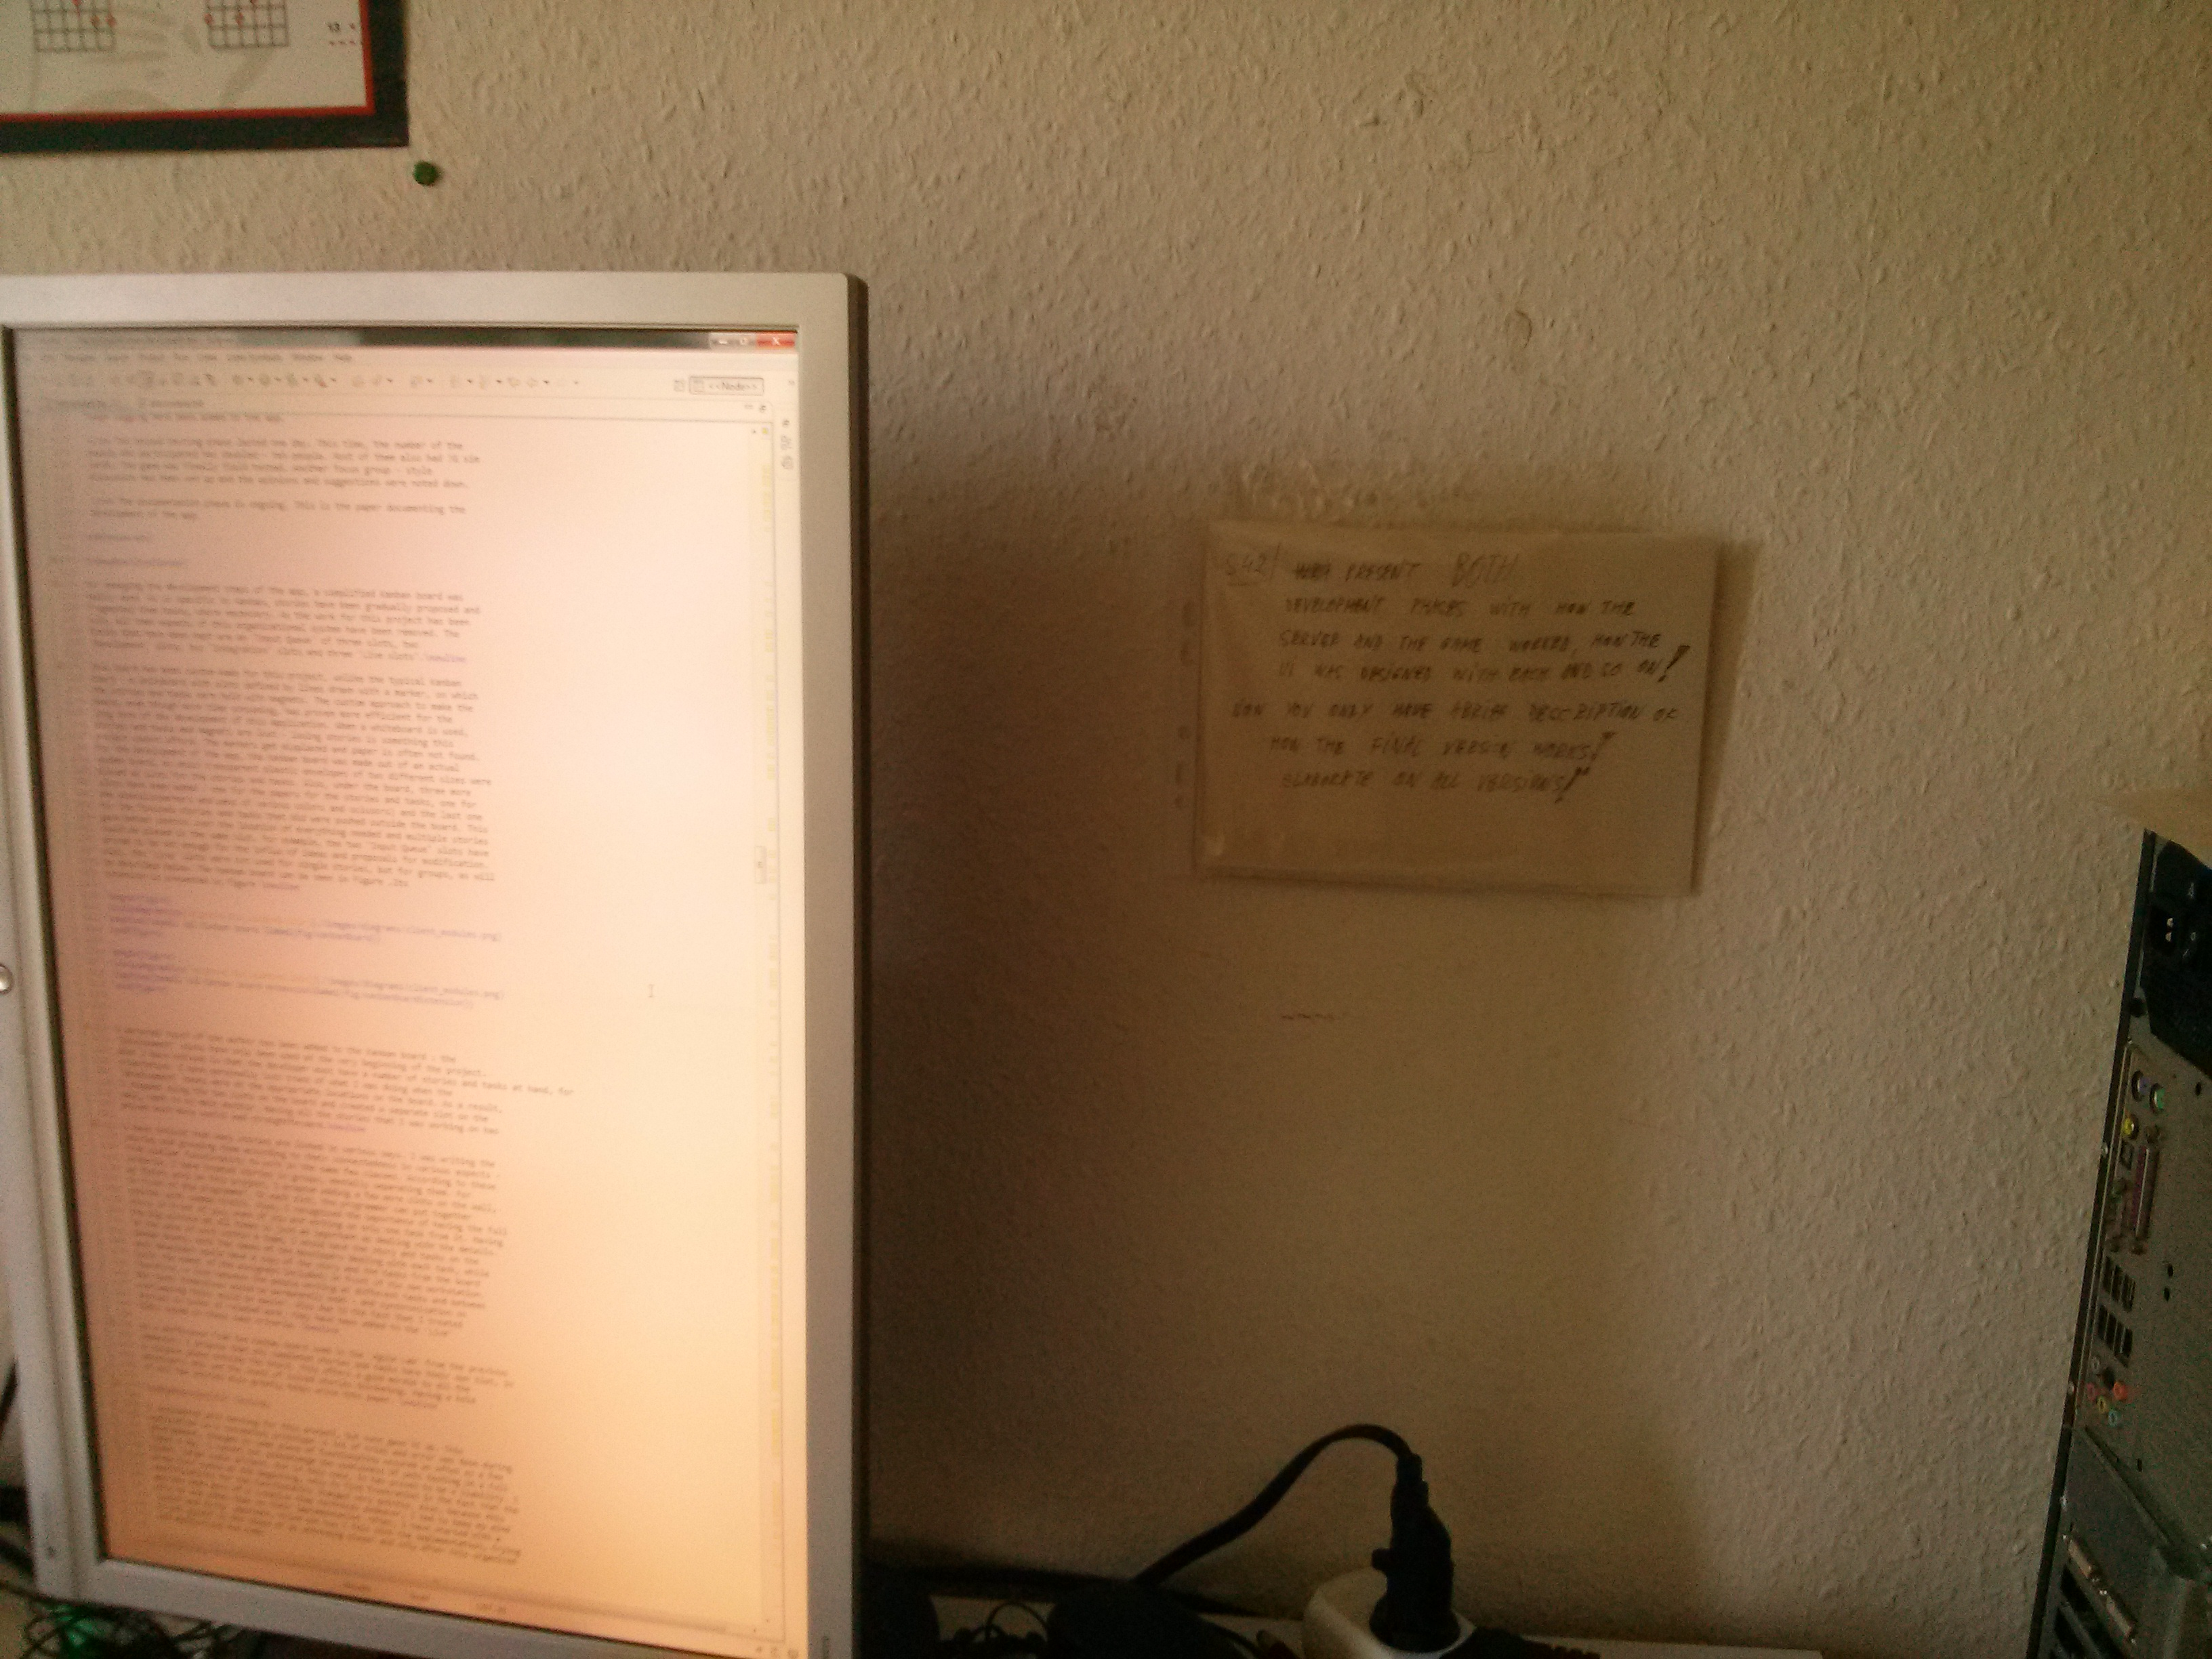
\includegraphics[height=3.5in,width=6.23in]{./images/kanban/kanban_board_extension.jpg}  
\caption{\small \sl Kanban board extension\label{fig:kanbanBoardExtension}}
\end{figure}


The Kanban board has been modified in one further aspect: As the 'Development'
slots have only been used at the very beginning of the project, they have been
brought closer to the programmer. The developer must have a number of stories
and tasks at hand, for orientation - it is easy to lose track of what must be
done, when delving into the unknown. As a result, the two slots on the board
have ceased to be used and a separate slot on the wall, next to the development
machine has been created. Having all the stories at hand has proven much more
useful and straightforward.\newline

Another observation is that many stories are linked in various ways.
During this project, stories have been grouped according to their connectedness
in various aspects - from similar functionality to work in the same few classes.
According to these criteria, stories have been treated in groups. For future
work on this project, we propose adding a few more slots on the wall, in front
of the programmer. In each slot, the programmer can put together stories with
common traits. Also, the importance of having the full story in front of the
developer has been noticed - even if one is working on only one task from it.
Having the big picture at all times is just as important as dealing with the
details. Therefore, for the case of work within a team, we bring the following
proposal: have the story and tasks on the Kanban board, with the names of the
developers dealing with each task, while each developer would have a copy of the
story and the tasks from the board (with the names of the assignees included) in
front of his own workstation. Therefore, a link between the people working at
different tasks and between the tasks themselves would be permanently kept - and
synchronization on overlapping tasks would be easier. Also due to the fact that
stories have been treated in bulks of related work, they have been added to the
'Live' slots based on these same criteria. \newline

Besides all, having all completed stories and tasks have their own slot, in
a visible place outside the board, has proven beneficial. It provides good
morale to the developer who sees the stack of solved stories thickening.
Having a hold of all the stories also greatly helped write this paper. \newline

\subsection{Unit Testing}

Unit testing has been considered for this project, but was soon given up. This
application is a conceptual prototype. A lot of trial and error was done during
development, changes to some pieces of functionality occured as often as a few
times a day. It is hard not to acknowledge the usefulness of unit testing in a
full blown, large scale project. But in this case, it has proven to be a
liability. At the beginning, writing unit tests has been attempted, only to be
abandoned in frustration -  the specifications for the functionality changed
very quickly. A lot of refactoring and hand testing each new piece of
functionality has kept the application mostly bug-free throughout the
development.

\subsection{Choosing the technologies}

The original plan was to develop and Android and iOS app, using a development
framework such as PhoneGap. This would assume Javascript / JQuery programming
for the UI and application backend. The communication was planned to be
established through Websockets. Therefore, for optimum performance, NodeJS was
to be used on the server side. For the location presentation, the Google Maps
API was to be used. 

\subsubsection{Unified vs. Native Frameworks}

Once an idea of how the game should look like was crystalized, a search was
made for unified frameworks for cross-platform mobile development. The first
choice was PhoneGap, which has been previously used by the author. The other
frameworks considered have been Titanium SDK, Sencha and Corona. The
multiplatform APIs offer the benefit of the 'code once, deploy everywhere'
philosophy, at the cost of performance \cite{nativevscrossplatform}
\cite{nativevscrossplatform2} \cite{nativevscrossplatform3}.
In this case, the approach of using a platform-agnostic framework is
disadvantageous. The discussion on which one is better can be resumed to the
conclusion that none of them is appropriate for the development of such a
game.\newline

And here are the reasons : 
\begin{enumerate}
  \item The game is fast-paced and will require a fast backend as well as a
  frontend that is as fast as possible. The cross-platform frameworks
  essentially interface only some of the native functionality and display the
  app through a webview - requiring Javascript or a Javascript-based framework
  for creating the interfaces. These frameworks have been previously tested by
  the author. The outcome has been disappointing. Qooxdoo, ExtJs and JQuery were
  tried out. Qooxdoo performs faster than the other two, but makes it very slow
  and tedious to develop a complex UI and almost impossible to add extra
  functionality. Still, it is slow for the purpose and feels nonnative. After
  reading a few articles that compare Phonegap, Titanium, Sencha and Corona, it
  has been concluded that with or without various advantages and disadvantages
  between them, they are all similar in performance - and therefore too slow for
  the development of this game.
  
  \item Developing native code can prove to be easier, as the Android
  development community is much larger than that of Phonegap developers, for
  example. The support is both more intensive and extensive for native
  platforms. 
  
\end{enumerate}

From this point on, the unified frameworks have been given up and a decision had
to be made between iOS and Android development. This was an easy choice: Android
develpment is free, while iOS development requires a paid developer account and
XCode runing on MacOS exclusively. Android was chosen.


\subsubsection{Communication Protocols}

A list of protocols have been proposed before beginning of this project: 

\begin{enumerate}
	\item WebRTC - A protocol that is to be part of the HTML 5 standard. It will be
	based on the RTP(Reliable Transport Protocol), which is the base for VoIP
	protocols and is itself based on UDP. It promises to be a very fast standard
	protocol, appropriate for audio and video streaming and massive multiplayer
	games.\cite{webrtc} It is still in draft format and there are no official
	implementations for it. Implementing the protocol itself is outside the scope
	of this project.
	\item WebSockets - A protocol that is part of the HTML 5 standard. It is a low
	latency TCP-based protocol that promisses to replace http in several types of
	web applications.\cite{websockets}
	\item TCP - One of the most intensely used two internet transport protocols in
	digital communication today. It is designed for transmission reliability.\cite{tcp}
	\item UDP - The other one of the most intensely used two internet
	transport-level protocols in digital communication today.\cite{udp}
	\item RTP - The protocol on which VoIP and WebRTC are based. It is based on UDP
	and it is designed for real-time streaming of data.\cite{rtp}
\end{enumerate}

Further on, when the design of the application was in progress, all unreliable
protocols have been discarded. TCP and Websockets were left in the discussion.
Initially, the use Websockets for the client-server communication was planned.
The reasoning behind it has two main arguments : 
\begin{enumerate}
  \item Websockets is an HTML5 protocol currently presented in draft by the
  IETF. This protocol provides reliable two-way communication between a server
  and a client and manages various complex issues or network features that come
  above TCP. This future standard is developed to replace HTTP and add
  functionality for technical aspects that HTTP was not covering. The reason for
  using Websockets for the client-server communication was that it promises to
  abstract a lot of protocol management issues, while offering speeds close to
  plain TCP. Also, for the game to run properly, UDP and its child protocols
  cannot be used - total reliability is required in the communication. 
  
  \item Websockets communication can be implemented in NodeJS, which is a
  framework well suited for fast-paced message exchanges and which has been
  proven more scalable than, for example, Apache Tomcat.
\end{enumerate}

As was decided to develop the server in NodeJS, the first choice was to use the
Socket.IO Websocket plugin. For the client side, Autobahn for Android was
chosen. The alternatives for Autobahn at that time were not free. After
developing a basic Websockets client with Autobahn for Android, communication
between the two was attempted. It did not work. After a search it was found out
that the protocol draft version that Socket.IO is using is different than that
used in Autobahn, and unlike Autobahn, Socket.IO uses an HTTP handshake for
establishing the connection. The Websocket-Node and ws NodeJS libraries for
Websocket communication were tried out afterwards. Neither were compatible with
Autobahn for Android. Then, Autobahn for Python was tried shortly and an
attempt to use Autobahn for Android in a Java project has failed. It was then
decided to give up Websockets and start off with pure TCP. Because writing code
in two different languages might be slower, the server has been written in Java.

\subsubsection{Google Maps API V1}

The first version of the app used Google Maps API V1. It has been chosen
because it had the most community support and the author had absolutely no
experience with Android development and the Google Maps API.  Unfortunately, the
Google Maps API and the Android Support Library cannot work together at the same
time, because they need to subclass different Fragment classes. Therefore, this
enforced the initial development to be done without the support library and
therefore the application has initially supported only Android versions equal or
higher than 3.0.

\subsubsection{Map Overlays}

The Google Maps V1 API supports the use of Overlay objects to draw on top
of the map. Most tutotials found online make use of the so-called
ItemizedOverlay, which enables easy integration of multiple location markers.
Using this Overlay subclass was attempted, but given up. Here are the
conclusions: \newline
\begin{enumerate}
  \item The ItemizedOverlay uses features that we may call 'magic'. The
  ItemizedOverlay object uses an ArrayList for storing the map markers as
  OverlayItem objects. It also needs a function that gives it the size of the
  ArrayList and redraws them automatically. This was bad on both the
  organizational aspect of the development and that of performance. Not all
  markers have to be redrawn at the same time.
  
  \item The fact that the markers are redrawn automatically has proven difficult
  to work with. For starters, there is no control over the draw process. Then,
  the OverlayItem objects cannot be stored in another data structure, such as a
  HashMap - which is used in keeping track of the players in the game.
  
  \item Because of its design, the ItemizedOverlay is fast, but useless for the
  purpose of this app. It was chosen to replace it with a custom Overlay.   
\end{enumerate}

As a replacement for the ItemizedOverlay, work on how to create a custom Overlay
that would fit the needs of the application was started. This has also permitted
the dynamic change of the marker icons, according to the needs of the game
mechanics and UI. Functionality was added for this particular feature. \newline

A real challenge was to add proper onTap() functionality for the custom Overlay.
The advantage of the already-given-up ItemizedOverlay was that it handled
position marker touch events. The new, custom overlay had no such thing
implemented. What was done was to get the pixel resolution of the screen, along
with pixel density data from the system and consider a 0.2 inch radius around
the center of the touch on the screen (this is what has been estimated to be
a circle to describe the tip of an average human adult finger). That 0.2 inch
radius in pixels has been translated in a radius, in meters, on the Google Map.
All markers inside that radius were considered and the closest to the center of
the touch was chosen. This made choosing a marker out of both crowded and loose
situations relatively easy and natural. The tutorial for this will be added as
an annex to the paper.\newline

\subsubsection{Google Maps API V2}

The use of the Google Maps API V1 ended when the absolute need to make the
application compatible with Android version 2.3, the most widespread version -
encompassing almost 50\% of the devices in use at the point of change. The
compatibility libraries require the use of a custom FragmentActivity and custom
Fragment, FragmentManager, FragmentTransaction objects. The Google Maps V1 API
requires a MapActivity to work. This comes into conflict with the
FragmentActivity. In a fortunate turn of events, the change has been done when a
total revamp of the game UI was also required.

\subsubsection{Google Maps API V1 vs. V2}

The migration to V2 is very destructive and at first feels quite unnatural. The
entire logic is changed. In V1, the map is rendered through a MapView object
that can be manipulated in a more direct and intuitive manner - lower level
access is both possible and needed. In contrast, the V2 map is accessed through
a GoogleMap object, which is no longer subclassing View. Therefore, it cannot be
manipulated in the same manner. Adding markers is done through the .addMarker()
method of the GoogleMap object. The same applies to drawing circles. Now lists
must be kept for all drawn objects, not for future redrawing, but for being able
to remove or change them. The entire Fragment object, along with a lot of
helper classes had to be rewritten completely. All methods helping out the
onTouch event for the custom Overlay were not necessary anymore. Also many
refresh workarounds were thrown away and in the process.


\subsubsection{Android development}

It must also be mentioned that learning how to program in Android was done while
developing. This was often a trial-and-error process, covered with the
author's personal takes on the tutorials found mostly on forums and blogs.

